\documentclass[11pt]{article}
\usepackage{graphicx}
\usepackage{multirow}
\usepackage{amsmath,amssymb,amsfonts}
\usepackage{amsthm}
\usepackage[title]{appendix}
\usepackage{xcolor}
\usepackage{textcomp}
\usepackage{booktabs}
\usepackage{listings}
\usepackage{url}
\usepackage[LGR,T1]{fontenc}
\usepackage[utf8]{inputenc}
\usepackage{alphabeta}
\usepackage[a4paper,margin=2.4cm]{geometry}
\usepackage{caption}
\usepackage{enumitem}
\usepackage[hidelinks]{hyperref}
\captionsetup{font=small,labelfont=bf}
\setlength{\parskip}{0.4em}
\setlength{\parindent}{0pt}
\newcommand{\euro}{\texteuro}
\definecolor{srcgray}{gray}{0.35}
\newcommand{\src}[1]{{\footnotesize\color{srcgray}[\textit{πηγή:} #1]}}

\title{\textbf{Κράτος Δικαίου, Ελευθερία του Τύπου και Λογοδοσία\\
Ελλάδα, 2010--2025:\\ Σχήμα Δεικτών Βασισμένο σε Αποδεικτικά Στοιχεία}\\[4pt]
\large Έκθεση Δομημένων Δεδομένων, «Παρακολούθηση»}
\author{Στιγμιότυπο Δεδομένων: 21 Ιουλίου 2026}
\date{}

\begin{document}
\maketitle

\begin{abstract}
\noindent
Η παρούσα έκθεση περιγράφει ένα ολοκληρωμένο, ελεγχόμενο από πηγές σχήμα δεικτών
(2010--2025) σχετικά με το κράτος δικαίου, την ελευθερία του Τύπου και τη θεσμική
λογοδοσία στην Ελλάδα. Περιλαμβάνει 20 πηγές, 630 αρχεία δεικτών (21 μεμονωμένοι
δείκτες), 64 αρχεία υποθέσεων βασισμένα σε αποδεικτικά στοιχεία και μια
αναπαραγώγιμη διαδικασία ενσωμάτωσης. Χαρακτηριστικά: Πρόκειται για αρχεία
αναζήτησης, όχι για δικαστικές αποφάσεις. Κάθε καταχώρηση περιλαμβάνει έναν
σύνδεσμο πηγής και μια ετικέτα κατάστασης (καταδικασμένος/ένοχος,
κατηγορούμενος/υπό έρευνα, μη επιβεβαιωμένος). Τα συνολικά πρότυπα δεν είναι
ομοιόμορφα. Έχει καταγραφεί σαφής επιδείνωση της ελευθερίας του Τύπου και του
κράτους δικαίου, ενώ οι δείκτες διαφθοράς έχουν δείξει μικτά ή σταθερά επίπεδα. Η
ερμηνεία γίνεται μόνο όταν πολλαπλές ανεξάρτητες πηγές καταλήγουν σε ένα συνεπές
συμπέρασμα και αναφέρεται ρητά στα τεκμηριωμένα αποτελέσματα.
\end{abstract}

\section{Πλαίσιο και Μεθοδολογία}

Αυτή η βάση δεδομένων είναι ένα αρχείο αναζήτησης, όχι μια κρίση. Κάθε καταχώρηση
έχει μια \texttt{source\_url} και μια ετικέτα κατάστασης:

\begin{itemize}[leftmargin=1.4em,itemsep=1pt]
\item \textsc{established} / \textsc{convicted}: τεκμηριωμένο ή δικαστικά κριμένο.
\item \textsc{alleged} / \textsc{under\_investigation}: αμφισβητούμενο· ισχύει το τεκμήριο αθωότητας.
\item \textsc{unverified}: αναφερόμενο, αλλά μη επιβεβαιωμένο.
\end{itemize}

Αυτό το εργαλείο δεν χρησιμοποιεί τη δική του αναπαράσταση. Απλώς καταγράφει αυτό
που υποδεικνύει η κύρια πηγή, το αποδίδει στο ίδρυμα που την καθόρισε και καταγράφει
τις αντικρούσεις. Η Πύλη Ελέγχου (Πύλη) προκαλεί την αποτυχία της δημιουργίας εάν
λείπει μια πηγή, η κατάσταση είναι άκυρη ή εάν εμφανίζεται μια πηγή τύπου Wikipedia.

\begin{table}[h]\centering
\caption{Μέγεθος Βάσης Δεδομένων και Πηγές}
\small
\begin{tabular}{@{}lll@{}}
\toprule
Αρχεία Στοιχείων & Αρχεία & Πηγές Αναφοράς \\ \midrule
Δείκτες (Χρονικές Σειρές) & 630 (21 στοιχεία) & RSF, V-Dem, TI, Παγκόσμια Τράπεζα WGI \\
Τεκμηριωμένα Αρχεία & 64 & EPPO, ΑΠΔΠΧ, Συμβούλιο της Ευρώπης, Αμνηστία, PEGA \\
Ιδιοκτησία Μέσων Ενημέρωσης & 9 & CMPF, Παρατηρητήριο Ιδιοκτησίας ΜΜΕ \\
Αστυνομική Βία & 9 & Αμνηστία, Δικαστικές Αποφάσεις \\
Αναφορές & 12 & MFRR, RSF \\
\bottomrule
\end{tabular}
\end{table}

Κατανομή Κατάστασης Αρχείων: Επιβεβαιωμένοι 50, Κατηγορούμενοι 8, Καταδικασμένοι 3,
Υπό Έρευνα 3. Δεν υπάρχουν αρχεία χωρίς συγκεκριμένες πηγές· δεν υπάρχουν πηγές
Wikipedia.

\section{Η θέση της Ελλάδας εντός των 27 χωρών της ΕΕ}

\begin{figure}[h]\centering
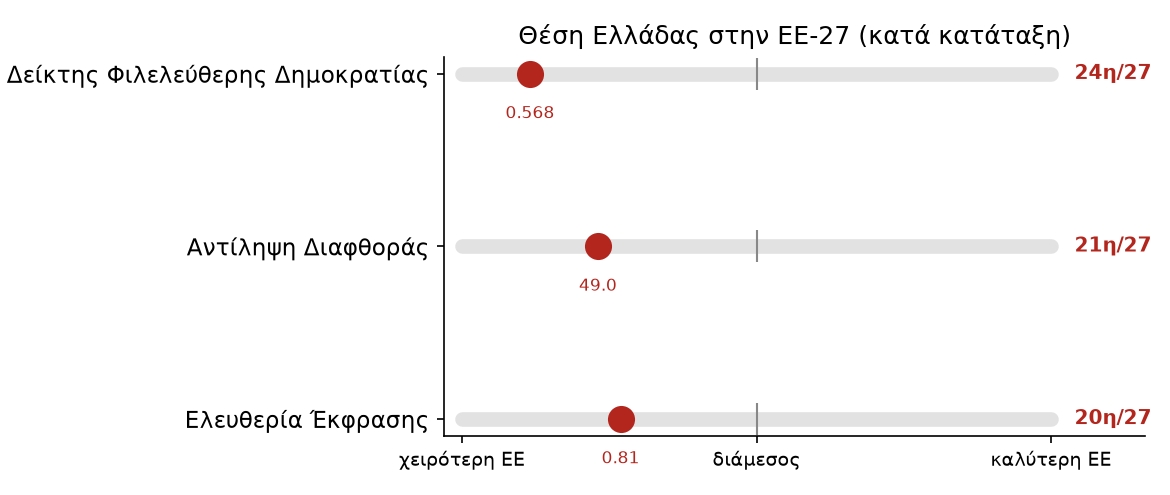
\includegraphics[width=0.82\linewidth]{fig_watchdog_eu.png}
\caption{Θέση της Ελλάδας ($\bullet$) σε σχέση με τον διάμεσο της ΕΕ-27 ($|$). Η
θέση των σημείων αντιστοιχεί στις τάξεις (δεξιά), αποτρέποντας έτσι τις παρεξηγήσεις
που προκαλούνται από την ασύμμετρη κατανομή των τιμών. \src{OWID/V-Dem/TI· Τελικό
σημείο \texttt{/eu-comparison}}}
\end{figure}

Η κατάταξη της Ελλάδας υπολογίζεται με βάση τις πραγματικές τιμές των 27 κρατών
μελών και δεν αποτελεί τεχνητά δημιουργημένο μέσο όρο. Η Ελλάδα βρίσκεται στο
κατώτερο τρίτο και για τους τρεις δείκτες. Ο Δείκτης Φιλελεύθερης Δημοκρατίας
κατατάσσεται 24ος από τις 27 χώρες, ο Δείκτης Αντίληψης Διαφθοράς (TI) κατατάσσεται
21ος από τις 27 χώρες και η Ελευθερία της Έκφρασης κατατάσσεται 20ός από τις 27
χώρες.

\section{Τάσεις Σύνθετου Δείκτη 2010--2025}

\begin{figure}[h]\centering
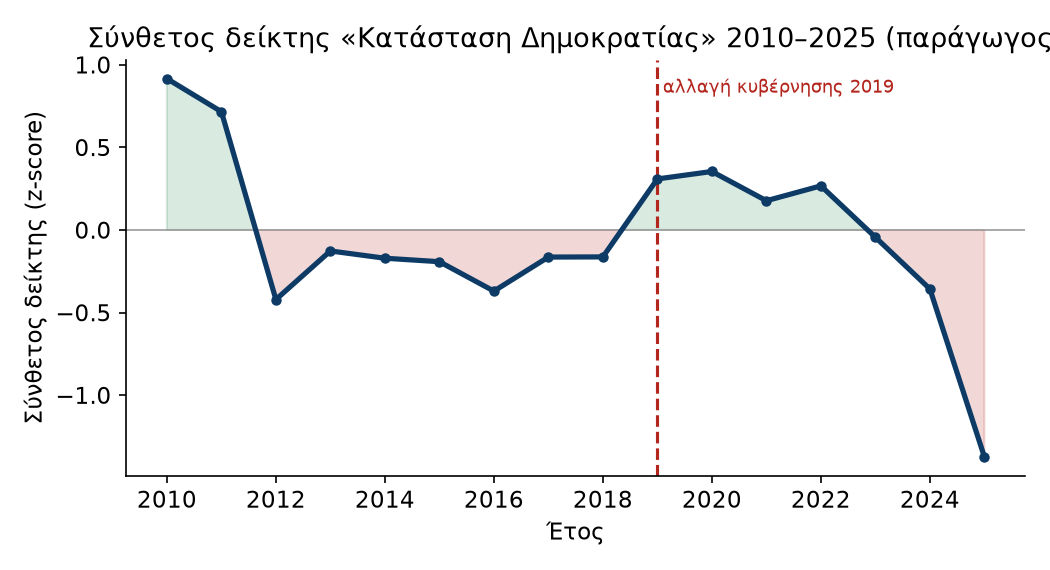
\includegraphics[width=0.78\linewidth]{fig_watchdog_composite.png}
\caption{Σύνθετος Δείκτης (z-score, RSF/V-Dem/TI/WGI 6 στοιχεία σταθμισμένα εξίσου).
Πρόκειται για ένα παράγωγο εργαλείο σύνοψης, όχι για επίσημη μέτρηση. \src{endpoint
\texttt{/composite-index}}}
\end{figure}

Ο Σύνθετος Δείκτης είναι ένα ρητά παράγωγο εργαλείο σύνοψης και κάθε στοιχείο
εμφανίζεται ξεχωριστά στην εφαρμογή. Η τάση μειώνεται από $+0{,}92\sigma$ (2010) σε
$-1{,}37\sigma$ (2025). Η γραμμή του 2019 υποδηλώνει αλλαγή καθεστώτος. Η ερμηνεία
της συσχέτισης αφήνεται στον αναγνώστη.

\section{Πριν / Μετά το 2019}

Τομή των χρονοσειρών που καταγράφηκαν ανά ημερομηνία (ουδέτερος υπολογισμός, καμία
αιτιώδης σχέση για την αλλαγή).

\begin{table}[h]\centering
\caption{Αλλαγές στους Δείκτες Διακυβέρνησης Πριν και Μετά το 2019}
\small
\begin{tabular}{@{}lccc@{}}
\toprule
Δείκτης & Πριν & Μετά & Αλλαγή \\ \midrule
Αποτελεσματικότητα της Κυβέρνησης (WGI) & 60,3 & 55,1 & $-5{,}2$ \\
Κράτος Δικαίου (WGI) & 63,6 & 62,1 & $-1{,}5$ \\
Φιλελεύθερη Δημοκρατία (V-Dem) & 0,76 & 0,57 & $-0{,}20$ \\
Ελευθερία Έκφρασης (V-Dem) & 0,91 & 0,81 & $-0{,}10$ \\
\bottomrule
\end{tabular}
\end{table}

Και οι τέσσερις δείκτες έχουν επιδεινωθεί.

\section{Λογοδοσία: 18 Υποθέσεις}

Σύμφωνα με τα αρχεία και τους φακέλους αστυνομικής βίας, τα αποτελέσματα χωρίζονται
σε 9 καταδικαστικές αποφάσεις, 7 εκκρεμείς υποθέσεις, 1 αθώα απόφαση και 1 μη
απαγγελία κατηγορητηρίου. Το «Ρολόι Ασυλίας» υπολογίζει τον αριθμό των ημερών που
έχουν παρέλθει για υποθέσεις χωρίς τελική έκβαση (π.χ. υπόθεση Νέας Σμύρνης περίπου
1.960 ημέρες, υπόθεση ναυαγίου Πύλου περίπου 1.130 ημέρες). Κάθε υπόθεση συνδέεται
με μια κύρια πηγή πληροφοριών.

\section{Ιδιοκτησία Μέσων Ενημέρωσης και Κρατική Διαφήμιση}

Εννέα δομές ιδιοκτησίας (όλες \texttt{is\_official=FALSE}, παρακολούθηση/πηγή
τύπου, αμφιλεγόμενο). Η κρατική διαφήμιση που σχετίζεται με την COVID-19 («Λίστα
Πέτσα», 19.832.132\,\euro, 2020) εμφανίζεται στην ακόλουθη ροή:
Ιδιοκτήτης~$\rightarrow$~Μέσα Ενημέρωσης. Ενώ καταγράφεται το συνολικό ποσό, οι
λεπτομέρειες ανά τύπο μέσου δεν έχουν αποκαλυφθεί ή συγκεντρωθεί. Παρουσιάζεται μόνο
η δομή ιδιοκτησίας· δεν παρέχονται ποσά ανά εταιρεία.

\section{Ουδετερότητα, Ερμηνεία και Όρια}
\begin{itemize}[leftmargin=1.4em,itemsep=1pt]
\item \textbf{Ουδέτερη Προοπτική:} Χρήση μόνο θεσμικά τεκμηριωμένων γεγονότων, με ετικέτες κατάστασης. Απαγορεύεται ο χαρακτηρισμός.
\item \textbf{Βάση Ερμηνείας:} Ελευθερία του Τύπου και κράτος δικαίου. Οι τομείς όπου οι RSF, V-Dem, το Συμβούλιο της Ευρώπης και η PEGA έχουν καταλήξει σε συναίνεση σχετικά με την επιδείνωση προσδιορίζονται ως τεκμηριωμένα αποτελέσματα έρευνας.
\item \textbf{Μη Βάση Ερμηνείας:} Οι αξιολογήσεις της διαφθοράς είναι μικτές και δεν εμφανίζεται καμία ενιαία αφήγηση παρακμής.
\item \textbf{Αποποίηση ευθύνης:} Ορισμένα θεσμικά υλικά / υλικά μέσων ενημέρωσης δεν επαληθεύονται σε πραγματικό χρόνο σε περιβάλλον sandbox (αυτό δεν σημαίνει ότι οι σύνδεσμοι είναι νεκροί). Οι δείκτες RSF πριν από το 2022 εξαιρούνται από τις άμεσες συγκρίσεις, καθώς χρησιμοποιούν αντίστροφες κλίμακες.
\end{itemize}

\section{Αναπαραγωγιμότητα και Παραπομπή}

Οι βάσεις δεδομένων μπορούν να ανακατασκευαστούν με μία μόνο εντολή. Τελικά σημεία:
\texttt{/eu-comparison}, \texttt{/composite-index}, \texttt{/before-after},
\texttt{/impunity}, \texttt{/network}, \texttt{/state-ad-flow}, \texttt{/dossier},
\texttt{/export/\{table\}}. Προτεινόμενη παραπομπή: \emph{Παρακολούθηση, τεκμηριωμένη βάση δεικτών, στιγμιότυπο 21 Ιουλίου 2026· πηγές όπως αναγράφονται ανά
στοιχείο.}

\begin{thebibliography}{9}
\bibitem{rsf} Reporters Without Borders (RSF), \emph{World Press Freedom Index}, \url{https://rsf.org}.
\bibitem{vdem} V-Dem Institute, \emph{Varieties of Democracy} dataset, \url{https://v-dem.net}.
\bibitem{ti} Transparency International, \emph{Corruption Perceptions Index}.
\bibitem{wgi} World Bank, \emph{Worldwide Governance Indicators}.
\bibitem{coe} Council of Europe, Platform for the protection of journalism.
\bibitem{pega} European Parliament, PEGA committee, spyware inquiry.
\bibitem{cmpf} Centre for Media Pluralism and Media Freedom (EUI), \emph{Media Pluralism Monitor}.
\end{thebibliography}

\end{document}
